\section{Knowledge-workers e carico cognitivo}
Secondo una definizione antecedente al 2007 i "lavoratori della conoscenza" ({\bf knowledge workers}) sono coloro che "manipolano direttamente dei simboli per creare un prodotto di conoscenza originale o per fornire valore aggiunto ad un prodotto già esistente".\newline
Il termine "knowledge workers" fu utilizzato per la prima volta nel 1959 da Peter Drucker nel libro "Landmarks of Tomorrow".\newline
In senso più ampio i Knowledge workers sono tutti coloro che trasformano la propria conoscenza professionale e i propri input conoscitivi in output di conoscenza con un valore aggiunto rispetto a quello di partenza \cite{knowledge_workers}.\newline
Questo tipo di lavoro consuma dunque principalmente risorse cognitive piuttosto che fisiche; suddette risorse inoltre vengono consumate non solo in contesto lavorativo, ma da praticamente ogni attività che viene svolta nel corso di una giornata.\newline
Dipendentemente dal tipo di attività svolta e da quanta familiarità si ha con essa la quantità di risorse mentali impiegata varia significativamente.\newline
Definiamo dunque il consumo di risorse mentali per una determinata attività come {\bf carico cognitivo}.\newline
Studi in materia evidenziano inoltre come l'incidenza del carico cognitivo e le performance di un individuo siano collegate anche all'affaticamento accumulato nel corso del tempo; un individuo che esegue un'attività in una condizione di stress otterrà risultati peggiori ed impiegando un maggiore sforzo rispetto allo stesso individuo che provenga da una situazione di relax.\newline
Questo fenomeno viene chiamato "affaticamento mentale" ({\bf Mental fatigue}) \cite{mental_fatigue}.\newline
Distinguiamo due tipi di Mental Fatigue:
\begin{itemize}
  \item \emph{Acute Mental Fatigue}\\
  {Questo tipo di affaticamento riguarda una circostanza con durata nel breve periodo; questa condizione può essere superata da un individuo attraverso del semplice riposo.}
  \item \emph{Chronic Mental Fatigue}\\
  {Si parla di affaticamento mentale cronico quando una condizione di stress per l'individuo viene protratta nel lungo periodo ed il riposo non è sufficiente a superare questa condizione. La permanenza di un individuo in questo stato aumenta drasticamente l'incidenza di un fenomeno chiamato {\bf Occupational Burnout} \cite{occupational_burnout}, la condizione in cui un individuo supera il proprio limite cognitivo con gravi conseguenze emotive, comportamentali e fisiche.}
\end{itemize}
\begin{figure}[H]
  \centering
  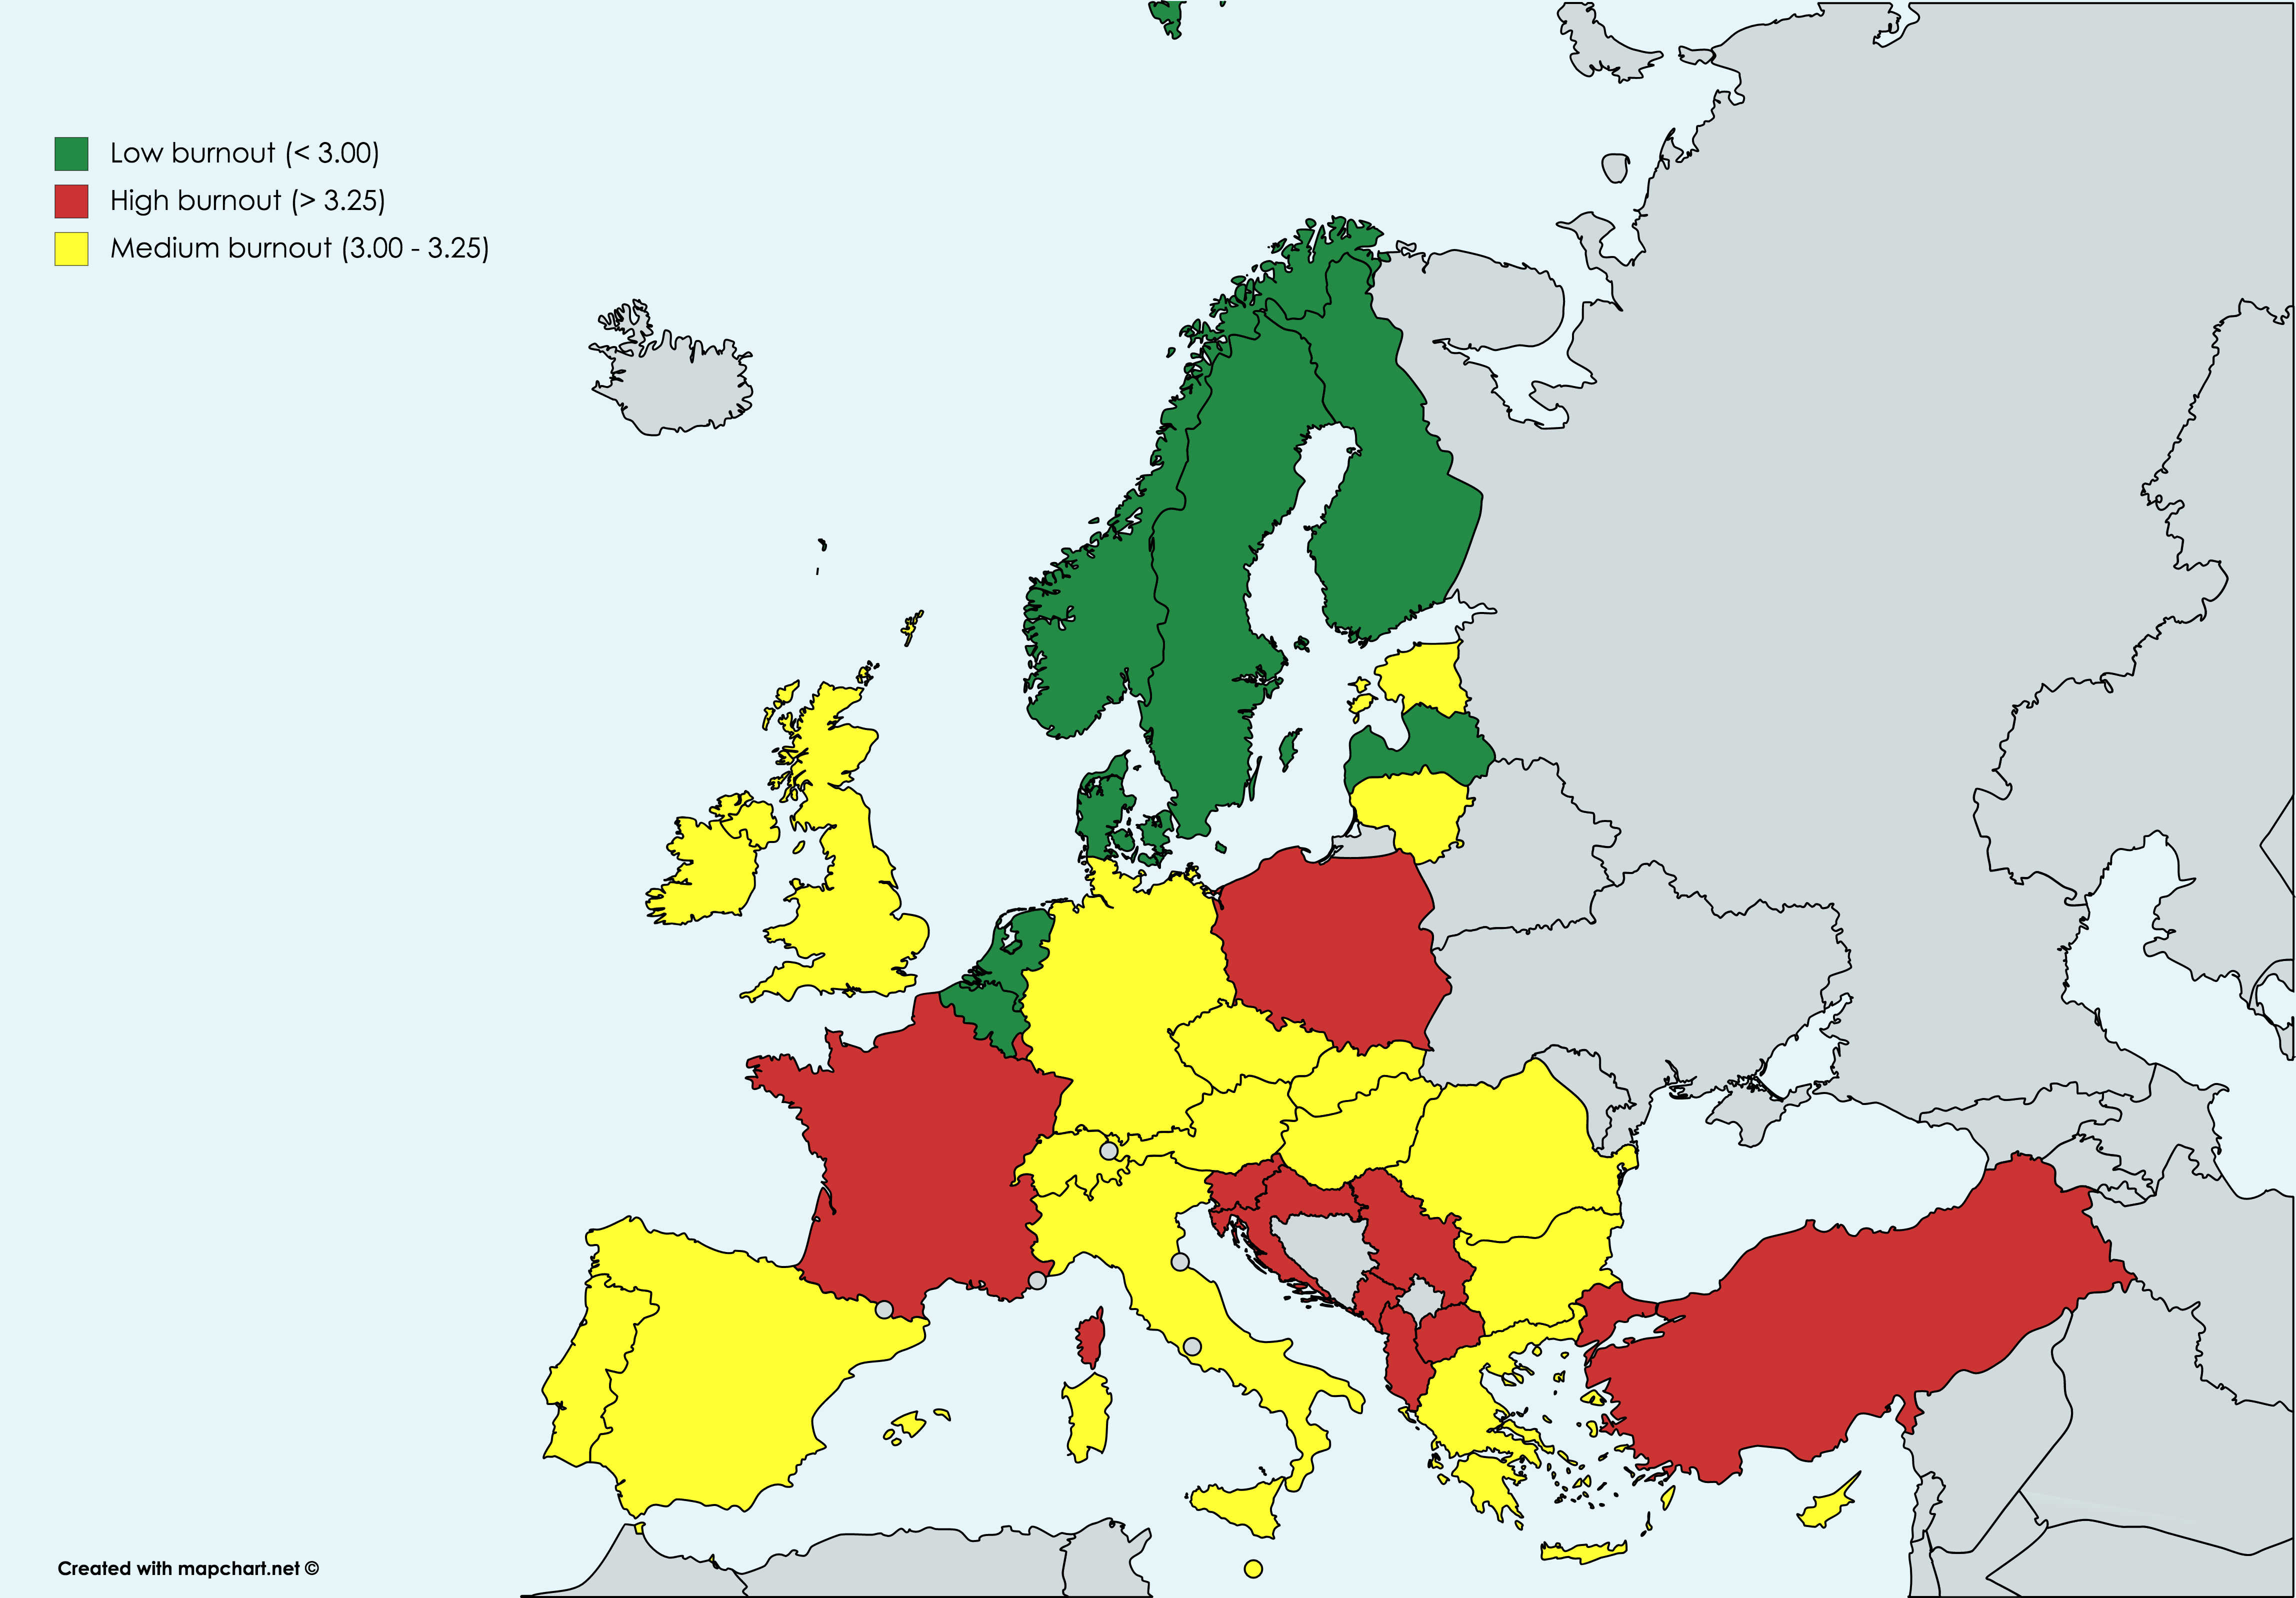
\includegraphics[width=0.75\textwidth]{img/burnout_eu_2015.png}
  \caption{Livello medio di Burnout in Europa(2015)[scala da 1 a 5] \cite{burnout_europa}}
\end{figure}
\vspace{15mm}
La gestione delle risorse mentali nell'era digitale dunque diventa un aspetto fondamentale per la salute dei lavoratori ed in generale di tutti gli individui.\newline
Una corretta gestione delle risorse mentali inoltre può incrementare drasticamente la qualità del lavoro prodotto, permettendo ad un individuo di raggiungere lo stato di {\bf Flow} \cite{flow}; questo stato si ottiene quando si dedica completa attenzione ad un'attività di cui si è appassionati ed in cui si è totalmente immersi.\newline
Durante il Flow le normali sensazioni che distraggono un individuo dal lavoro (come affaticamento, fame, stimoli fisici ed ambientali) scompaiono permettendo la massima resa nel lavoro impiegando il minimo sforzo.